\chapter{Scales, axes and legends}\label{cha:scales}

\section{Introduction}

Scales control the mapping from data to aesthetics. They take your data
and turn it into something that you can perceive visually: e.g., size,
colour, position or shape. Scales also provide the tools you use to read
the plot: the axes and legends (collectively known as guides). Formally,
each scale is a function from a region in data space (the domain of the
scale) to a region in aesthetic space (the range of the range). The
domain of each scale corresponds to the range of the variable supplied
to the scale, and can be continuous or discrete, ordered or unordered.
The range consists of the concrete aesthetics that you can perceive and
that R can understand: position, colour, shape, size and line type. If
you blinked when you read that scales map data both to position and
colour, you are not alone. The notion that the same kind of object is
used to map data to positions and symbols strikes some people as
unintuitive. However, you will see the logic and power of this notion as
you read further in the chapter.

The process of scaling takes place in three steps, transformation,
training and mapping, and is described in
\hyperref[sec:how-scales-work]{how scales work}. Without a scale, there
is no way to go from the data to aesthetics, so a scale is required for
every aesthetic used on the plot. It would be tedious to manually add a
scale every time you used a new aesthetic, so whenever a scale is needed
ggplot will add a default. You can generate many plots without knowing
how scales work, but understanding scales and learning how to manipulate
them will give you much more control. Default scales and how to override
them are described in \hyperref[sec:scale-usage]{scale usage}.

Scales can be roughly divided into four categories: position scales,
colour scales, the manual discrete scale and the identity scale. The
common options and most important uses are described in
\hyperref[sec:scale-details]{scale details}. The section focusses on
giving you a high-level overview of the options available, rather than
expanding on every detail in depth. Details about individual parameters
are included in the online documentation.

The other important role of each scale is to produce a \textbf{guide}
that allows the viewer to perform the inverse mapping, from aesthetic
space to data space, and read values off the plot. For position
aesthetics, the axes are the guides; for all other aesthetics, legends
do the job. Unlike other plotting systems, you have little direct
control over the axis or legend: there is no \texttt{gglegend()} or
\texttt{ggaxis()} to call to modify legends or axes. Instead, all
aspects of the guides are controlled by parameters of the scale. Axes
and legends are discussed in \hyperref[sec:guides]{legends and axes}.

\hyperref[sec:scale-resources]{More resources} concludes the chapter
with pointers to other academic work that discusses some of the things
you need to keep in mind when assigning variables to aesthetics.

\hyperdef{}{sec:how-scales-work}{\section{How scales
work}\label{sec:how-scales-work}}

To describe how scales work, we will first describe the domain (the data
space) and the range (the aesthetic space), and then outline the process
by which one is mapped to the other.

Since an input variable is either discrete or continuous, the domain is
either a set of values (stored as a factor, character vector or logical
vector) \indexf{Discrete variables} or an interval on the real line
(stored as a numeric vector of length 2). For example, in the mammals
sleep dataset (\texttt{msleep}), the domain of the discrete variable
\texttt{vore} is \{carni, herbi, omni, insecti\}, and the domain of the
continuous variable \texttt{bodywt} is \([0.005, 6654]\). We often think
of these as data ranges, but here we are focussing on their nature as
input to the scale, i.e., as a domain of a function.
\index{Data!msleep@\texttt{msleep}}

The range can also be discrete or continuous. For discrete scales, it is
a vector of aesthetic values corresponding to the input values. For
continuous scales, it is a 1d path through some more complicated space.
For example, a colour gradient interpolates linearly from one colour to
another. The range is either specified by the user when the scale is
created, or by the scale itself.

The process of mapping the domain to the range includes the following
stages:

\begin{itemize}
\itemsep1pt\parskip0pt\parsep0pt
\item
  \textbf{transformation}: (for continuous domain only). It is often
  useful to display a transformation of the data, such as a logarithm or
  square root. Transformations are described in more depth in
  \hyperref[sub:scale-position]{position scales}.
  \index{Scales!transformation}
\end{itemize}

After any transformations have been applied, the statistical summaries
for each layer are computed based on the transformed data. This ensures
that a plot of \(\log(x)\) vs. \(\log(y)\) on linear scales looks the
same as \(x\) vs. \(y\) on log scales.

\begin{itemize}
\itemsep1pt\parskip0pt\parsep0pt
\item
  \textbf{training}: During this key stage, the domain of the scale is
  learned. Sometimes learning the domain of a scale is extremely
  straightforward: In a plot with only one layer, representing only raw
  data, it consists of determining the minimum and maximum values of a
  continuous variable (after transformation), or listing the unique
  levels of a categorical variable. However, often the domain must
  reflect multiple layers across multiple datasets in multiple panels.
  For example, imagine a scale that will be used to create an axis; the
  minimum and maximum values of the raw data in the first layer and the
  statistical summary in the second layer are likely to be different,
  but they must all eventually be drawn on the same plot.
  \index{Scales!training}
\end{itemize}

The domain can also be specified directly, overriding the training
process, by manually setting the domain of the scale with the
\texttt{limits} argument, as described in
\hyperref[sec:scale-usage]{scale usage}. Any values outside of the
domain of the scale will be mapped to \texttt{NA}.

\begin{itemize}
\itemsep1pt\parskip0pt\parsep0pt
\item
  \textbf{mapping}: We now know the domain and we already knew the range
  before we started this process, so the last thing to do is to apply
  the scaling function that maps data values to aesthetic values.
  \index{Scales!mapping}
\end{itemize}

We have left a few stages out of this description of the process for
simplicity. For example, we haven't discussed the role faceting plays in
training, and we have also ignored position adjustments. Nevertheless
this description is accurate, and you should come back to it if you are
confused about what scales are doing in your plot.

\hyperdef{}{sec:scale-usage}{\section{Usage}\label{sec:scale-usage}}

Every aesthetic has a default scale that is added to the plot whenever
you use that aesthetic. These are listed in Table
\ref{tbl:default-scales}. The scale depends on the variable type:
continuous (numeric) or discrete (factor, logical, character). If you
want to change the default scales see \texttt{set\_default\_scale},
described in \hyperref[sub:customise-scales]{scales}.

Default scales are added when you initialise the plot and when you add
new layers. This means it is possible to get a mismatch between the
variable type and the scale type if you later modify the underlying data
or aesthetic mappings. When this happens you need to add the correct
scale yourself. The following example illustrates the problem and
solution. \index{Scales!defaults}

\begin{Shaded}
\begin{Highlighting}[]
\NormalTok{plot <-}\StringTok{ }\KeywordTok{qplot}\NormalTok{(cty, hwy, }\DataTypeTok{data =} \NormalTok{mpg)}
\NormalTok{plot}

\CommentTok{# This doesn't work because there is a mismatch between the}
\CommentTok{# variable type and the default scale}
\NormalTok{plot +}\StringTok{ }\KeywordTok{aes}\NormalTok{(}\DataTypeTok{x =} \NormalTok{drv)}

\CommentTok{# Correcting the default manually resolves the problem.}
\NormalTok{plot +}\StringTok{ }\KeywordTok{aes}\NormalTok{(}\DataTypeTok{x =} \NormalTok{drv) +}\StringTok{ }\KeywordTok{scale_x_discrete}\NormalTok{()}
\end{Highlighting}
\end{Shaded}

To add a different scale or to modify some features of the default
scale, you must construct a new scale and then add it to the plot using
\texttt{+}. \indexc{+} All scale constructors have a common naming
scheme. They start with \texttt{scale\_}, followed by the name of the
aesthetic (e.g., \texttt{colour\_}, \texttt{shape\_} or \texttt{x\_}),
and finally by the name of the scale (e.g., \texttt{gradient},
\texttt{hue} or \texttt{manual}). For example, the name of the default
scale for the colour aesthetic based on discrete data is
\texttt{scale\_colour\_hue()}, and the name of the Brewer colour scale
for fill colour is \texttt{scale\_fill\_brewer()}. \index{Scales!adding}

\begin{table}
  \begin{center}
  \begin{tabular}{p{1in}p{1in}p{1in}}
    \toprule
    Aesthetic & Discrete & Continuous \\
    \midrule
    Colour and fill & brewer \newline grey \newline \textbf{hue} \newline identity \newline manual & \textbf{gradient} \newline gradient2 \newline gradientn \\[0.5em]
    Position (x, y) & \textbf{discrete} & \textbf{continuous}\newline date \\[0.5em]
    Shape & \textbf{shape} \newline identity \newline manual  \\[0.5em]
    Line type & \textbf{linetype} \newline identity \newline manual \\[0.5em]
    Size & identity \newline manual & \textbf{size} \\
    \bottomrule
  \end{tabular}
  \end{center}
  \caption{Scales, by aesthetic and variable type.  Default scales are emboldened. The default scale varies depending on whether the variable is continuous or discrete.  Shape and line type do not have a default continuous scale; size does not have a default discrete scale.}
  \label{tbl:default-scales}
\end{table}

The following code illustrates this process. We start with a plot that
uses the default colour scale, and then modify it to adjust the
appearance of the legend, and then use a different colour scale. The
results are shown in Figure \ref{fig:scale-adjust}.

\begin{Shaded}
\begin{Highlighting}[]
\NormalTok{p <-}\StringTok{ }\KeywordTok{qplot}\NormalTok{(sleep_total, sleep_cycle, }\DataTypeTok{data =} \NormalTok{msleep, }\DataTypeTok{colour =} \NormalTok{vore)}
\NormalTok{p }
\CommentTok{# Explicitly add the default scale}
\NormalTok{p +}\StringTok{ }\KeywordTok{scale_colour_hue}\NormalTok{()}

\CommentTok{# Adjust parameters of the default, here changing the appearance }
\CommentTok{# of the legend}
\NormalTok{p +}\StringTok{ }\KeywordTok{scale_colour_hue}\NormalTok{(}\StringTok{"What does}\CharTok{\textbackslash{}n}\StringTok{it eat?"}\NormalTok{, }
   \DataTypeTok{breaks =} \KeywordTok{c}\NormalTok{(}\StringTok{"herbi"}\NormalTok{, }\StringTok{"carni"}\NormalTok{, }\StringTok{"omni"}\NormalTok{, }\OtherTok{NA}\NormalTok{), }
   \DataTypeTok{labels =} \KeywordTok{c}\NormalTok{(}\StringTok{"plants"}\NormalTok{, }\StringTok{"meat"}\NormalTok{, }\StringTok{"both"}\NormalTok{, }\StringTok{"don't know"}\NormalTok{))}

\CommentTok{# Use a different scale}
\NormalTok{p +}\StringTok{ }\KeywordTok{scale_colour_brewer}\NormalTok{(}\DataTypeTok{palette =} \StringTok{"Set1"}\NormalTok{)}
\end{Highlighting}
\end{Shaded}

\begin{figure}

{\centering \includegraphics[width=0.49\linewidth]{figures/scalesscale-adjust-1} \includegraphics[width=0.49\linewidth]{figures/scalesscale-adjust-2} \includegraphics[width=0.49\linewidth]{figures/scalesscale-adjust-3} \includegraphics[width=0.49\linewidth]{figures/scalesscale-adjust-4} 

}

\caption{Adjusting the default parameters of a scale. (Top left) The plot with default scale. (Top right) Adding the default scale by hand doesn't change the appearance of the plot. (Bottom left) Adjusting the parameters of the scale to tweak the legend. (Bottom right) Using a different colour scale: Set1 from the ColorBrewer colours.\label{fig:scale-adjust}}
\end{figure}

\hyperdef{}{sec:scale-details}{\section{Scale
details}\label{sec:scale-details}}

Scales can be divided roughly into four separate groups:

\begin{itemize}
\itemsep1pt\parskip0pt\parsep0pt
\item
  Position scales, used to map continuous, discrete and date-time
  variables onto the plotting region and to construct the corresponding
  axes.
\item
  Colour scales, used to map continuous and discrete variables to
  colours.
\item
  Manual scales, used to map discrete variables to your choice of symbol
  size, line type, shape or colour, and to create the corresponding
  legend.
\item
  The identity scale, used to plot variable values directly to the
  aesthetic rather than mapping them. For example, if the variable you
  want to map to symbol colour is itself a vector of colours, you want
  to render those values directly rather than mapping them to some other
  colours.
\end{itemize}

\noindent  This section describes each group in more detail. Precise
details about individual scales can be found in the documentation,
within R (e.g., \texttt{?scale\_brewer}), or online at
\url{http://docs.ggplot2.org/}.

\subsection{Common arguments}\label{sub:scale-arguments}

The following arguments are common to all scales.

\begin{itemize}
\itemsep1pt\parskip0pt\parsep0pt
\item
  \texttt{name}: sets the label which will appear on the axis or legend.
  You can supply text strings (using \texttt{\textbackslash{}n} for line
  breaks) or mathematical expressions (as described by
  \texttt{?plotmath}). Because tweaking these labels is such a common
  task, there are three helper functions to save you some typing:
  \texttt{xlab}, \texttt{ylab} and \texttt{labs}. Their use is
  demonstrated in the code below and results are shown in Figure
  \ref{fig:legend-names}. \index{Axis!labels} \index{Legend!title}
  \index{Scales!names}
\end{itemize}

\begin{Shaded}
\begin{Highlighting}[]
\NormalTok{p <-}\StringTok{ }\KeywordTok{qplot}\NormalTok{(cty, hwy, }\DataTypeTok{data =} \NormalTok{mpg, }\DataTypeTok{colour =} \NormalTok{displ)}
\NormalTok{p}
\NormalTok{p +}\StringTok{ }\KeywordTok{scale_x_continuous}\NormalTok{(}\StringTok{"City mpg"}\NormalTok{)}
\NormalTok{p +}\StringTok{ }\KeywordTok{xlab}\NormalTok{(}\StringTok{"City mpg"}\NormalTok{)}
\NormalTok{p +}\StringTok{ }\KeywordTok{ylab}\NormalTok{(}\StringTok{"Highway mpg"}\NormalTok{)}
\NormalTok{p +}\StringTok{ }\KeywordTok{labs}\NormalTok{(}\DataTypeTok{x =} \StringTok{"City mpg"}\NormalTok{, }\DataTypeTok{y =} \StringTok{"Highway"}\NormalTok{, }\DataTypeTok{colour =} \StringTok{"Displacement"}\NormalTok{)}
\NormalTok{p +}\StringTok{ }\KeywordTok{xlab}\NormalTok{(}\KeywordTok{expression}\NormalTok{(}\KeywordTok{frac}\NormalTok{(miles, gallon)))}
\end{Highlighting}
\end{Shaded}

\begin{figure}

{\centering \includegraphics[width=0.32\linewidth]{figures/scaleslegend-names-1} \includegraphics[width=0.32\linewidth]{figures/scaleslegend-names-2} \includegraphics[width=0.32\linewidth]{figures/scaleslegend-names-3} \includegraphics[width=0.32\linewidth]{figures/scaleslegend-names-4} \includegraphics[width=0.32\linewidth]{figures/scaleslegend-names-5} \includegraphics[width=0.32\linewidth]{figures/scaleslegend-names-6} 

}

\caption{A demonstration of the different forms legend title can take.\label{fig:legend-names}}
\end{figure}

\begin{itemize}
\itemsep1pt\parskip0pt\parsep0pt
\item
  \texttt{limits}: fixes the domain of the scale. Continuous scales take
  a numeric vector of length two; discrete scales take a character
  vector. If limits are set, no training of the data will be performed.
  See \hyperref[sub:scale-position]{position scales} for shortcuts.
  \index{Axis!limits} \index{Scales!limits}
\end{itemize}

Limits are useful for removing data you don't want displayed in a plot
(i.e., setting limits that are smaller than the full range of data), and
for ensuring that limits are consistent across multiple plots intended
to be compared (i.e., setting limits that are larger or smaller than
some of the default ranges).

Any value not in the domain of the scale is discarded: for an
observation to be included in the plot, each aesthetic must be in the
domain of each scale. This discarding occurs before statistics are
calculated.

\begin{itemize}
\itemsep1pt\parskip0pt\parsep0pt
\item
  \texttt{breaks} and \texttt{labels}: \texttt{breaks} controls which
  values appear on the axis or legend, i.e., what values tick marks
  should appear on an axis or how a continuous scale is segmented in a
  legend. \texttt{labels} specifies the labels that should appear at the
  breakpoints. If \texttt{labels} is set, you must also specify
  \texttt{breaks}, so that the two can be matched up correctly.
  \index{Axis!breaks} \index{Axis!labels} \index{Legend!keys}
\end{itemize}

To distinguish breaks from limits, remember that breaks affect what
appears on the axes and legends, while limits affect what appears on the
plot. See Figure \ref{fig:breaks_vs_limits} for an illustration. The
first column uses the default settings for both breaks and limits, which
are \texttt{limits = c(4, 8)} and \texttt{breaks = 4:8}. In the middle
column, the breaks have been reset: the plotted region is the same, but
the tick positions and labels have shifted. In the right column, it is
the limits which have been redefined, so much of the data now falls
outside the plotting region.

\begin{Shaded}
\begin{Highlighting}[]
\NormalTok{p <-}\StringTok{ }\KeywordTok{qplot}\NormalTok{(cyl, wt, }\DataTypeTok{data =} \NormalTok{mtcars)}
\NormalTok{p}
\NormalTok{p +}\StringTok{ }\KeywordTok{scale_x_continuous}\NormalTok{(}\DataTypeTok{breaks =} \KeywordTok{c}\NormalTok{(}\FloatTok{5.5}\NormalTok{, }\FloatTok{6.5}\NormalTok{))}
\NormalTok{p +}\StringTok{ }\KeywordTok{scale_x_continuous}\NormalTok{(}\DataTypeTok{limits =} \KeywordTok{c}\NormalTok{(}\FloatTok{5.5}\NormalTok{, }\FloatTok{6.5}\NormalTok{))}
\NormalTok{p <-}\StringTok{ }\KeywordTok{qplot}\NormalTok{(wt, cyl, }\DataTypeTok{data =} \NormalTok{mtcars, }\DataTypeTok{colour =} \NormalTok{cyl)}
\NormalTok{p}
\NormalTok{p +}\StringTok{ }\KeywordTok{scale_colour_gradient}\NormalTok{(}\DataTypeTok{breaks =} \KeywordTok{c}\NormalTok{(}\FloatTok{5.5}\NormalTok{, }\FloatTok{6.5}\NormalTok{))}
\NormalTok{p +}\StringTok{ }\KeywordTok{scale_colour_gradient}\NormalTok{(}\DataTypeTok{limits =} \KeywordTok{c}\NormalTok{(}\FloatTok{5.5}\NormalTok{, }\FloatTok{6.5}\NormalTok{))}
\end{Highlighting}
\end{Shaded}

\begin{figure}

{\centering \includegraphics[width=0.32\linewidth]{figures/scalesbreaks_vs_limits-1} \includegraphics[width=0.32\linewidth]{figures/scalesbreaks_vs_limits-2} \includegraphics[width=0.32\linewidth]{figures/scalesbreaks_vs_limits-3} \includegraphics[width=0.32\linewidth]{figures/scalesbreaks_vs_limits-4} \includegraphics[width=0.32\linewidth]{figures/scalesbreaks_vs_limits-5} \includegraphics[width=0.32\linewidth]{figures/scalesbreaks_vs_limits-6} 

}

\caption{The difference between breaks and limits. (Left) default plot with \texttt{limits = c(4, 8), breaks = 4:8}, (middle) \texttt{breaks = c(5.5,6.5)} and (right) \texttt{limits = c(5.5 ,6.5)}. The effect on the x axis (top) and colour legend (bottom)\label{fig:breaks_vs_limits}}
\end{figure}

\begin{itemize}
\itemsep1pt\parskip0pt\parsep0pt
\item
  \textbf{formatter}: if no labels are specified the formatter will be
  called on each break to produce the label. Useful formatters for
  continuous scales are \texttt{comma}, \texttt{percent},
  \texttt{dollar} and \texttt{scientific}, and for discrete scales is
  \texttt{abbreviate}. \index{Axis!formatting}
\end{itemize}

\hyperdef{}{sub:scale-position}{\subsection{Position
scales}\label{sub:scale-position}}

Every plot must have two position scales, one for the horizontal
position (the x scale) and one for the vertical position (the y scale).
\texttt{ggplot} comes with continuous, discrete (for factor, character
and logical vectors) and date scales. Each of these transform the data
in a slightly different way, and generate a slightly different type of
axis. The following sections describe each type in more detail.
\index{Scales!position} \index{Positioning!scales}

A common task for all position axes is changing the axis limits. Because
this is such a common task, \texttt{ggplot} provides a couple of helper
functions to save you some typing: \texttt{xlim} and \texttt{ylim}.
These functions inspect their input and then create the appropriate
scale, as follows: \index{Axis!limits} \index{Scales!limits}
\indexf{xlim} \indexf{ylim} \index{Limits|see{Axis, limits}}

\begin{itemize}
\itemsep1pt\parskip0pt\parsep0pt
\item
  \texttt{xlim(10, 20)}: a continuous scale from 10 to 20
\item
  \texttt{ylim(20, 10)}: a reversed continuous scale from 20 to 10
\item
  \texttt{xlim("a", "b", "c")}: a discrete scale
\item
  \texttt{xlim(as.Date(c("2008-05-01", "2008-08-01")))}: a date scale
  from May 1 to August 1 2008.
\end{itemize}

These limits do not work in the same way as \texttt{xlim} and
\texttt{ylim} in base or lattice graphics. In \texttt{ggplot}, to be
consistent with the other scales, any data outside the limits is not
plotted and not included in the statistical transformation. This means
that setting the limits is not the same as visually zooming in to a
region of the plot. To do that, you need to use the \texttt{xlim} and
\texttt{ylim} arguments to \texttt{coord\_cartesian()}, described in
\hyperref[sub:cartesian]{cartesian coordinate systems}. This performs
purely visual zooming and does not affect the underlying data.
\index{Zooming}

By default, the limits of position scales extend a little past the range
of the data. This ensures that the data does not overlap the axes. You
can control the amount of expansion with the \texttt{expand} argument.
This parameter should be a numeric vector of length two. The first
element gives the multiplicative expansion, and the second the additive
expansion. If you don't want any extra space, use
\texttt{expand = c(0, 0)}. \index{Axis!expansion}

\subsubsection{Continuous}\label{ssub:scale-continuous}

The most common continuous position scales are
\texttt{scale\_x\_continuous()} and \texttt{scale\_y\_continuous()},
which map data to the x and y axis. \index{Scales!position!continuous}
The most interesting variations are produced using transformations.
Every continuous scale takes a \texttt{trans} argument, allowing the
specification of a variety of transformations, both linear and
non-linear. The transformation is carried out by a `transformer,' which
describes the transformation, its inverse, and how to draw the labels.
Table \ref{tbl:common-trans} lists some of the more common transformers.
\index{Transformation!scales} \indexf{scale_x_continuous}
\indexf{scale_y_continuous} \index{Scales!continuous}

\begin{table}
  \centering
  \begin{tabular}{lll}
    \toprule
    Name & Function $f(x)$ & Inverse $f^{-1}(y)$ \\
    \midrule
    asn       & $\tanh^{-1}(x)$ & $\tanh(y)$ \\
    exp       & $e ^ x$         & $\log(y)$  \\
    identity  & $x$             & $y$        \\
    log       & $\log(x)$       & $e ^ y$    \\
    log10     & $\log_{10}(x)$  & $10 ^ y$   \\
    log2      & $\log_2(x)$     & $2 ^ y$    \\
    logit     & $\log(\frac{x}{1 - x})$ & $\frac{1}{1 + e(y)} $ \\
    pow10     & $10^x$          & $\log_{10}(y) $ \\
    probit    & $\Phi(x)$       & $\Phi^{-1}(y)$ \\
    recip     & $x^{-1}$        & $y^{-1}$ \\
    reverse   & $-x$            & $-y$     \\
    sqrt      & $x^{1/2}$       & $y ^ 2$  \\
    % power     & $\frac{x^p - 1}{p * sgn(values - 1)}$ & $|values| * p + 1 $ 
    \bottomrule
  \end{tabular}
  \caption{List of built-in transformers.}
  \label{tbl:common-trans}
\end{table}

Transformations are most often used to modify position scales, so there
are shortcuts for x, y and z scales: \texttt{scale\_x\_log10()} is
equivalent to \texttt{scale\_x\_continuous(trans = "log10")}. The
\texttt{trans} argument works for any continuous scale, including the
colour gradients described below, but the shortcuts only exist for
position scales. \index{Log transform} \indexf{scale_x_log10}
\indexf{scale_y_log10}

Of course, you can also perform the transformation yourself. For
example, instead of using \texttt{scale\_x\_log10()}, you could plot
\texttt{log10(x)}. That produces an identical result inside the plotting
region, but the axis and tick labels won't be the same. If you use a
transformed scale, the axes will be labelled in the original data space.
In both cases, the transformation occurs before the statistical summary.
Figure \ref{fig:trans} illustrates this difference with the following
code. \index{Transformation!data}

\begin{Shaded}
\begin{Highlighting}[]
\KeywordTok{qplot}\NormalTok{(}\KeywordTok{log10}\NormalTok{(carat), }\KeywordTok{log10}\NormalTok{(price), }\DataTypeTok{data =} \NormalTok{diamonds)}
\KeywordTok{qplot}\NormalTok{(carat, price, }\DataTypeTok{data =} \NormalTok{diamonds) +}\StringTok{ }
\StringTok{  }\KeywordTok{scale_x_log10}\NormalTok{() +}\StringTok{ }\KeywordTok{scale_y_log10}\NormalTok{()}
\end{Highlighting}
\end{Shaded}

\begin{figure}

{\centering \includegraphics[width=0.49\linewidth]{figures/scalestrans-1} \includegraphics[width=0.49\linewidth]{figures/scalestrans-2} 

}

\caption{A scatterplot of diamond price vs. carat illustrating the difference between log transforming the scale (left) and log transforming the data (right).  The plots are identical, but the axis labels are different.\label{fig:trans}}
\end{figure}

Transformers are also used in \texttt{coord\_trans()}, where the
transformation occurs after the statistic has been calculated, and
affects the shape of the graphical object drawn on the plot.
\texttt{coord\_trans()} is described in more detail in
\hyperref[sub:cartesian]{cartesian coordinate systems}.

\subsubsection{Date and time}\label{ssub:scale-date}

Dates and times are basically continuous values, but with special ways
of labelling the axes. Currently, only dates of class \texttt{date} and
times of class \texttt{POSIXct} are supported. If your dates are in a
different format you will need to convert them with \texttt{as.Date()}
or \texttt{as.POSIXct()}. \index{Date} \index{Time}
\index{Scales!date-time} \indexf{scale_x_datetime}

There are three arguments that control the appearance and location of
the ticks for date axes: \texttt{major}, \texttt{minor} and
\texttt{format}. Generally, the scale does a pretty good job of choosing
the defaults, but if you need to tweak them the details are as follows:

\begin{itemize}
\itemsep1pt\parskip0pt\parsep0pt
\item
  The \texttt{major} and \texttt{minor} arguments specify the position
  of major and minor breaks in terms of date units, years, months,
  weeks, days, hours, minutes and seconds, and can be combined with a
  multiplier. For example, \texttt{major = "2 weeks"} will place a major
  tick mark every two weeks. If not specified, the date scale has some
  reasonable default for choosing them automatically.
\item
  The \texttt{format} argument specifies how the tick labels should be
  formatted. Table\textasciitilde{}\ref{tbl:dates} lists the special
  characters used to display components of a date. For example, if you
  wanted to display dates of the form 14/10/1979, you would use the
  string \texttt{"\%d/\%m/\%y"}. \index{Time series!date formatting}
\end{itemize}

\begin{table}
  \begin{center}
  \begin{tabular}{ll}
    \toprule
    Code & Meaning \\
    \midrule
    \verb|%S| & second (00-59)\\
    \verb|%M| & minute (00-59)\\
    \verb|%l| & hour, in 12-hour clock (1-12)\\
    \verb|%I| & hour, in 12-hour clock (01-12)\\
    \verb|%H| & hour, in 24-hour clock (00-23)\\
    \verb|%a| & day of the week, abbreviated (Mon-Sun)\\
    \verb|%A| & day of the week, full (Monday-Sunday)\\
    \verb|%e| & day of the month (1-31)\\
    \verb|%d| & day of the month (01-31)\\
    \verb|%m| & month, numeric (01-12)\\
    \verb|%b| & month, abbreviated (Jan-Dec)\\
    \verb|%B| & month, full (January-December)\\
    \verb|%y| & year, without century (00-99)\\
    \verb|%Y| & year, with century (0000-9999)\\
    \bottomrule
    
  \end{tabular}
  \end{center}
  \caption{Common data formatting codes, adapted from the documentation of \texttt{strptime}.  Listed from shortest to longest duration.}
  \label{tbl:dates}
\end{table}

The code below generates the plots in Figure \ref{fig:date-scale},
illustrating some of these parameters.

\begin{Shaded}
\begin{Highlighting}[]
\NormalTok{plot <-}\StringTok{ }\KeywordTok{qplot}\NormalTok{(date, psavert, }\DataTypeTok{data =} \NormalTok{economics, }\DataTypeTok{geom =} \StringTok{"line"}\NormalTok{) +}\StringTok{ }
\StringTok{  }\KeywordTok{ylab}\NormalTok{(}\StringTok{"Personal savings rate"}\NormalTok{) +}
\StringTok{  }\KeywordTok{geom_hline}\NormalTok{(}\DataTypeTok{xintercept =} \DecValTok{0}\NormalTok{, }\DataTypeTok{colour =} \StringTok{"grey50"}\NormalTok{)}
\NormalTok{plot}
\KeywordTok{library}\NormalTok{(}\StringTok{"scales"}\NormalTok{) }\CommentTok{# to access breaks/formatting functions}
\NormalTok{plot +}\StringTok{ }\KeywordTok{scale_x_date}\NormalTok{(}
  \DataTypeTok{labels =} \KeywordTok{date_format}\NormalTok{(}\StringTok{"%Y"}\NormalTok{),}
  \DataTypeTok{breaks =} \KeywordTok{date_breaks}\NormalTok{(}\StringTok{"5 years"}\NormalTok{)}
\NormalTok{)}
\NormalTok{plot +}\StringTok{ }\KeywordTok{scale_x_date}\NormalTok{(}
  \DataTypeTok{limits =} \KeywordTok{as.Date}\NormalTok{(}\KeywordTok{c}\NormalTok{(}\StringTok{"2004-01-01"}\NormalTok{, }\StringTok{"2005-01-01"}\NormalTok{)),}
  \DataTypeTok{labels =} \KeywordTok{date_format}\NormalTok{(}\StringTok{"%Y-%m-%d"}\NormalTok{)}
\NormalTok{)}
\end{Highlighting}
\end{Shaded}

\begin{figure}

{\centering \includegraphics[width=0.32\linewidth]{figures/scalesdate-scale-1} \includegraphics[width=0.32\linewidth]{figures/scalesdate-scale-2} \includegraphics[width=0.32\linewidth]{figures/scalesdate-scale-3} 

}

\caption{A time series of personal savings rate. (Left) The default appearance, (middle) breaks every 10 years, and (right) scale restricted to 2004, with YMD date format. Measurements are recorded at the end of each month.\label{fig:date-scale}}
\end{figure}

\subsubsection{Discrete}\label{ssub:scale-discrete}

Discrete position scales map the unique values of their input to
integers. The order of the result can be controlled by the
\texttt{breaks} argument, and levels can be dropped with the
\texttt{limits} argument (or by using \texttt{xlim()} or
\texttt{ylim()}). Because it is often useful to place labels and other
annotations on intermediate positions on the plot, discrete position
scales also accept continuous values. If you have not adjusted the
breaks or limits, the numerical position of a factor level can be
calculated with \texttt{as.numeric()}: the values are placed on integers
starting at 1. \index{Scales!position!discrete}
\indexf{scale_x_discrete} \indexf{scale_y_discrete}
\index{Scales!discrete}

\subsection{Colour}\label{sub:scale-colour}

After position, probably the most commonly used aesthetic is colour.
There are quite a few different ways of mapping values to colours: three
different gradient based methods for continuous values, and two methods
for mapping discrete values. But before we look at the details of the
different methods, it's useful to learn a little bit of colour theory.
Colour theory is complex because the underlying biology of the eye and
brain is complex, and this introduction will only touch on some of the
more important issues. An excellent more detailed exposition is
available online at \url{http://tinyurl.com/clrdtls}. \index{Colour}
\index{Scales!colour}

At the physical level, colour is produced by a mixture of wavelengths of
lights. To know a colour completely we need to know the complete mixture
of wavelengths, but fortunately for us the human eye only has three
different colour receptors, and so we can summarise any colour with just
three numbers. You may be familiar with the rgb encoding of colour
space, which defines a colour by the intensities of red, green and blue
light needed to produce it. One problem with this space is that it is
not perceptually uniform: the two colours that are one unit apart may
look similar or very different depending on where in the colour space
they. This makes it difficult to create a mapping from a continuous
variable to a set of colours. There have been many attempts to come up
with colours spaces that are more perceptually uniform. We'll use a
modern attempt called the hcl colour space, which has three components
of \textbf{h} ue, \textbf{c} hroma and \textbf{l} uminance:
\index{Colour!spaces}

\begin{itemize}
\itemsep1pt\parskip0pt\parsep0pt
\item
  Hue is a number between 0 and 360 (an angle) which gives the
  ``colour'' of the colour: like blue, red, orange, etc.
\item
  Luminance is the lightness of the colour. A luminance of 0 produces
  black, and a luminance of 1 produces white.
\item
  Chroma is the purity of a colour. A chroma of 0 is grey, and the
  maximum value of chroma varies with luminance.
\end{itemize}

The combination of these three components does not produce a simple
geometric shape. Figure \ref{fig:hcl} attempts to show the 3d shape of
the space. Each slice is a constant luminance (brightness) with hue
mapped to angle and chroma to radius. You can see the centre of each
slice is grey and the colours get more intense as they get closer to the
edge.

\begin{figure}[htbp]
  \centering
    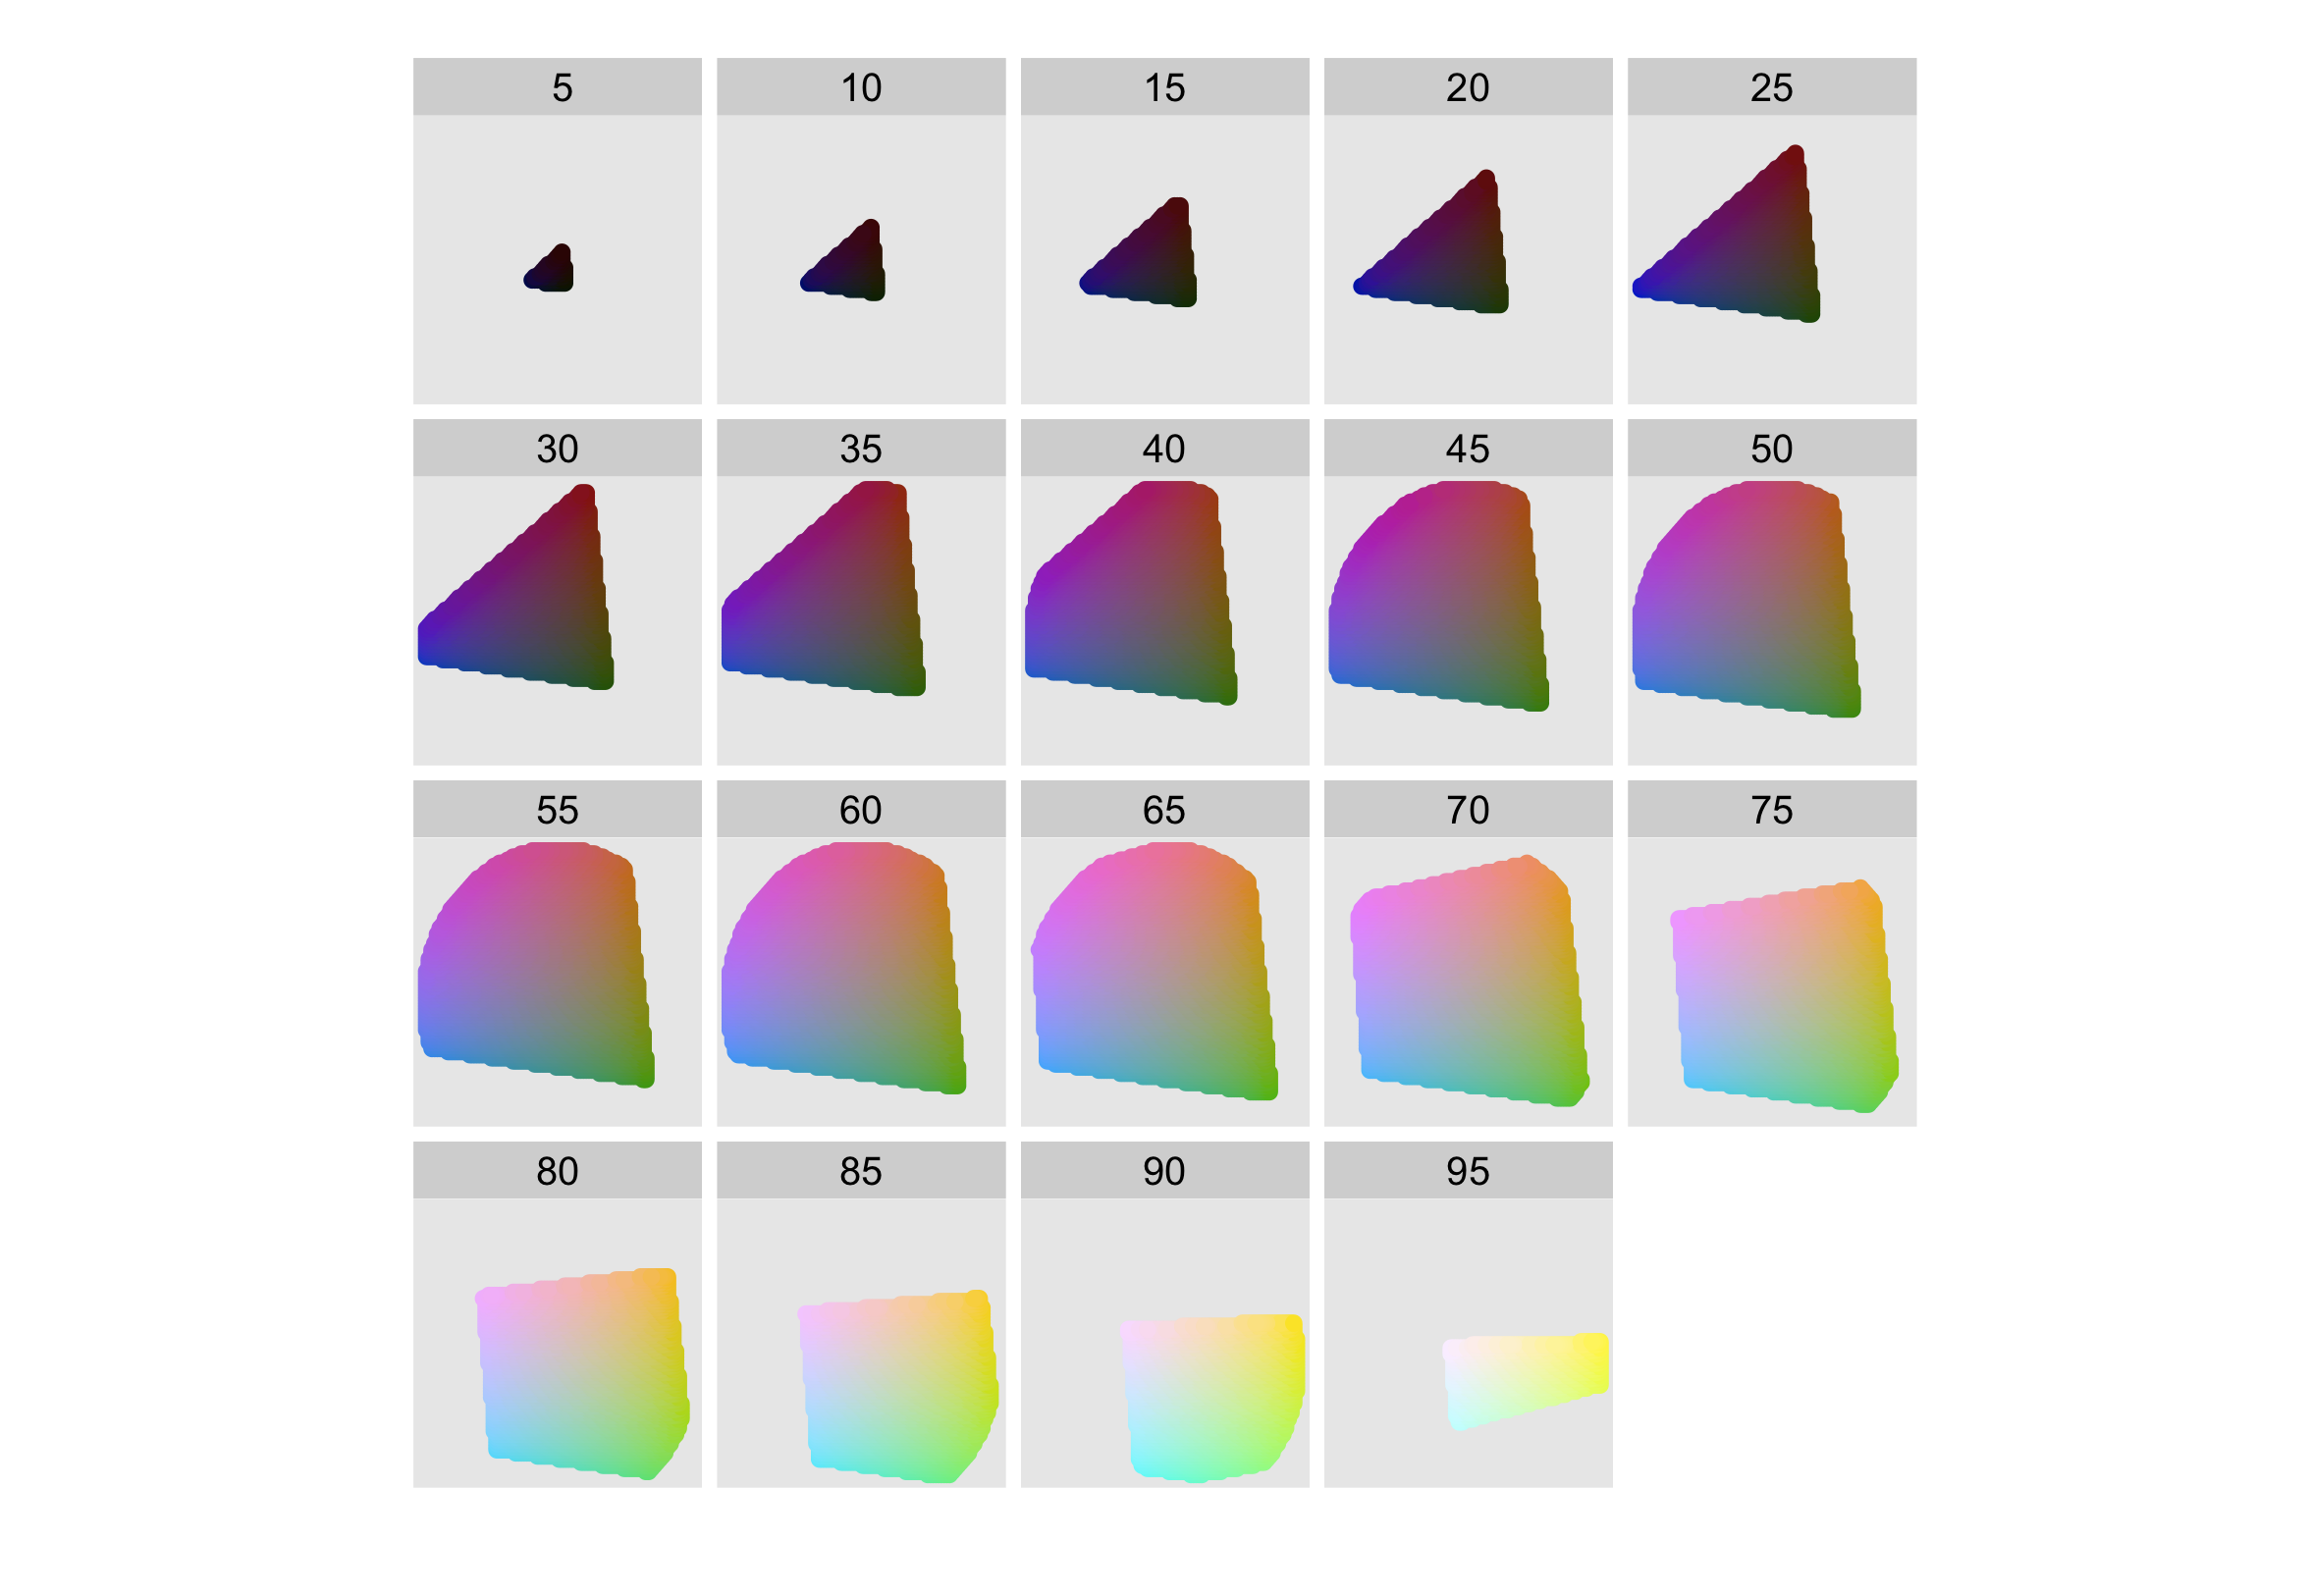
\includegraphics[width=\linewidth]{diagrams/hcl-space}
  \caption{The shape of the hcl colour space.  Hue is mapped to angle, chroma to radius and each slice shows a different luminance.  The hcl space is a pretty odd shape, but you can see that colours near the centre of each slice are grey, and as you move towards the edges they become more intense.  Slices for luminance 0 and 100 are omitted because they would, respectively, be a single black point and a single white point.}
  \label{fig:hcl}
\end{figure}

An additional complication is that many people (\textasciitilde{}10\% of
men) do not possess the normal complement of colour receptors and so can
distinguish fewer colours than usual. \index{Colour!blindness} In brief,
it's best to avoid red-green contrasts, and to check your plots with
systems that simulate colour blindness. Visicheck is one online
solution. Another alternative is the \textbf{dichromat} package (Lumley
2007) which provides tools for simulating colour blindness, and a set of
colour schemes known to work well for colour-blind people. You can also
help people with colour blindness in the same way that you can help
people with black-and-white printers: by providing redundant mappings to
other aesthetics like size, line type or shape.

All of the scales discussed in the following sections work with border
(\texttt{colour}) and fill (\texttt{fill}) colour aesthetics.

\subsubsection{Continuous}\label{ssub:colour-continuous}

There are three types of continuous colour gradients, based on the
number of colours in the gradient: \index{Colour!gradients}
\index{Scales!colour!gradient}

\begin{itemize}
\itemsep1pt\parskip0pt\parsep0pt
\item
  \texttt{scale\_colour\_gradient()} and
  \texttt{scale\_fill\_gradient()}: a two-colour gradient, low-high.
  Arguments \texttt{low} and \texttt{high} control the colours at either
  end of the gradient. \indexf{scale_colour_gradient}
  \indexf{scale_fill_gradient}
\item
  \texttt{scale\_colour\_gradient2()} and
  \texttt{scale\_fill\_gradient2()}: a three-colour gradient,
  low-med-high. As well as \texttt{low} and \texttt{high} colours, these
  scales also have a \texttt{mid} colour for the colour of the midpoint.
  The midpoint defaults to 0, but can be set to any value with the
  \texttt{midpoint} argument. This is particularly useful for creating
  diverging colour schemes.\indexf{scale_colour_gradient2}
  \indexf{scale_fill_gradient2}
\item
  \texttt{scale\_colour\_gradientn()} and
  \texttt{scale\_fill\_gradientn()}: a custom n-colour gradient. This
  scale requires a vector of colours in the \texttt{colours} argument.
  Without further arguments these colours will be evenly spaced along
  the range of the data. If you want the values to be unequally spaced,
  use the \texttt{values} argument, which should be between 0 and 1 if
  \texttt{rescale} is true (the default), or within the range of the
  data is \texttt{rescale} is false.
\end{itemize}

Colour gradients are often used to show the height of a 2d surface. In
the following example we'll use the surface of a 2d density estimate of
the \texttt{faithful} dataset (Azzalini and Bowman 1990), which records
the waiting time between eruptions and during each eruption for the Old
Faithful geyser in Yellowstone Park. Figure \ref{fig:gradient} shows
three gradients applied to this data, created with the following code.
Note the use of limits: this parameter is common to all scales.

\begin{Shaded}
\begin{Highlighting}[]
\NormalTok{f2d <-}\StringTok{ }\KeywordTok{with}\NormalTok{(faithful, MASS::}\KeywordTok{kde2d}\NormalTok{(eruptions, waiting, }
  \DataTypeTok{h =} \KeywordTok{c}\NormalTok{(}\DecValTok{1}\NormalTok{, }\DecValTok{10}\NormalTok{), }\DataTypeTok{n =} \DecValTok{50}\NormalTok{))}
\NormalTok{df <-}\StringTok{ }\KeywordTok{with}\NormalTok{(f2d, }\KeywordTok{cbind}\NormalTok{(}\KeywordTok{expand.grid}\NormalTok{(x, y), }\KeywordTok{as.vector}\NormalTok{(z)))}
\KeywordTok{names}\NormalTok{(df) <-}\StringTok{ }\KeywordTok{c}\NormalTok{(}\StringTok{"eruptions"}\NormalTok{, }\StringTok{"waiting"}\NormalTok{, }\StringTok{"density"}\NormalTok{)}
\NormalTok{erupt <-}\StringTok{ }\KeywordTok{ggplot}\NormalTok{(df, }\KeywordTok{aes}\NormalTok{(waiting, eruptions, }\DataTypeTok{fill =} \NormalTok{density)) +}
\StringTok{  }\KeywordTok{geom_tile}\NormalTok{() +}
\StringTok{  }\KeywordTok{scale_x_continuous}\NormalTok{(}\DataTypeTok{expand =} \KeywordTok{c}\NormalTok{(}\DecValTok{0}\NormalTok{, }\DecValTok{0}\NormalTok{)) +}\StringTok{ }
\StringTok{  }\KeywordTok{scale_y_continuous}\NormalTok{(}\DataTypeTok{expand =} \KeywordTok{c}\NormalTok{(}\DecValTok{0}\NormalTok{, }\DecValTok{0}\NormalTok{))}
\NormalTok{erupt +}\StringTok{ }\KeywordTok{scale_fill_gradient}\NormalTok{(}\DataTypeTok{limits =} \KeywordTok{c}\NormalTok{(}\DecValTok{0}\NormalTok{, }\FloatTok{0.04}\NormalTok{))}
\NormalTok{erupt +}\StringTok{ }\KeywordTok{scale_fill_gradient}\NormalTok{(}\DataTypeTok{limits =} \KeywordTok{c}\NormalTok{(}\DecValTok{0}\NormalTok{, }\FloatTok{0.04}\NormalTok{), }
  \DataTypeTok{low =} \StringTok{"white"}\NormalTok{, }\DataTypeTok{high =} \StringTok{"black"}\NormalTok{) }
\NormalTok{erupt +}\StringTok{ }\KeywordTok{scale_fill_gradient2}\NormalTok{(}\DataTypeTok{limits =} \KeywordTok{c}\NormalTok{(-}\FloatTok{0.04}\NormalTok{, }\FloatTok{0.04}\NormalTok{), }
  \DataTypeTok{midpoint =} \KeywordTok{mean}\NormalTok{(df$density)) }
\end{Highlighting}
\end{Shaded}

\begin{figure}

{\centering \includegraphics[width=0.32\linewidth]{figures/scalesgradient-1} \includegraphics[width=0.32\linewidth]{figures/scalesgradient-2} \includegraphics[width=0.32\linewidth]{figures/scalesgradient-3} 

}

\caption{Density of eruptions with three colour schemes. (Left) Default gradient colour scheme, (middle) customised gradient from white to black and (right) 3 point gradient with midpoint set to the mean density.\label{fig:gradient}}
\end{figure}

To create your own custom gradient, use
\texttt{scale\_colour\_gradientn()}. This is useful if you have colours
that are meaningful for your data (e.g., black body colours or standard
terrain colours), or you'd like to use a palette produced by another
package. The following code and Figure \ref{fig:colorspace} shows
palettes generated from routines in the \textbf{colorspace} package.
(Zeileis, Hornik, and Murrell 2008) describes the philosophy behind
these palettes and provides a good introduction to some of the
complexities of creating good colour scales. \index{Colour!palettes}
\indexf{scale_colour_gradientn} \indexf{scale_fill_gradientn}

\begin{Shaded}
\begin{Highlighting}[]
\KeywordTok{library}\NormalTok{(}\StringTok{"colorspace"}\NormalTok{)}
\NormalTok{fill_gradn <-}\StringTok{ }\NormalTok{function(pal) \{}
  \KeywordTok{scale_fill_gradientn}\NormalTok{(}\DataTypeTok{colours =} \KeywordTok{pal}\NormalTok{(}\DecValTok{7}\NormalTok{), }\DataTypeTok{limits =} \KeywordTok{c}\NormalTok{(}\DecValTok{0}\NormalTok{, }\FloatTok{0.04}\NormalTok{))}
\NormalTok{\}}
\NormalTok{erupt +}\StringTok{ }\KeywordTok{fill_gradn}\NormalTok{(rainbow_hcl)}
\NormalTok{erupt +}\StringTok{ }\KeywordTok{fill_gradn}\NormalTok{(diverge_hcl)}
\NormalTok{erupt +}\StringTok{ }\KeywordTok{fill_gradn}\NormalTok{(heat_hcl)}
\end{Highlighting}
\end{Shaded}

\begin{figure}

{\centering \includegraphics[width=0.32\linewidth]{figures/scalescolorspace-1} \includegraphics[width=0.32\linewidth]{figures/scalescolorspace-2} \includegraphics[width=0.32\linewidth]{figures/scalescolorspace-3} 

}

\caption{Gradient colour scales using perceptually well-formed palettes produced by the \textbf{colorspace} package.  From left to right: sequential, diverging and heat hcl palettes.  Each scale is produced with \texttt{scale\_fill\_gradientn} with \texttt{colours} set to \texttt{rainbow\_hcl(7)}, \texttt{diverge\_hcl(7)} and \texttt{heat\_hcl(7)}.\label{fig:colorspace}}
\end{figure}

\subsubsection{Discrete}\label{ssub:colour-discrete}

There are two colour scales for discrete data, one which chooses colours
in an automated way, and another which makes it easy to select from
hand-picked sets.

The default colour scheme, \texttt{scale\_colour\_hue()}, picks evenly
spaced hues around the hcl colour wheel. This works well for up to about
eight colours, but after that it becomes hard to tell the different
colours apart. Another disadvantage of the default colour scheme is that
because the colours all have the same luminance and chroma, when you
print them in black and white, they all appear as an identical shade of
grey. \index{Colour!discrete scale} \indexf{scale_colour_hue}

An alternative to this algorithmic scheme is to use the ColorBrewer
colours, \url{http://colorbrewer2.org/}. These colours have been hand
picked to work well in a wide variety of situations, although the focus
is on maps and so the colours tend to work better when displayed in
large areas. For categorical data, the palettes most of interest are
`Set1' and `Dark2' for points and `Set2', `Pastel1', `Pastel2' and
`Accent' for areas. Use \texttt{RColorBrewer::display.brewer.all()} to
list all palettes. Figure \ref{fig:brewer-pal} shows three of these
palettes applied to points and bars, created with the following code.
\index{Colour!Brewer} \indexf{scale_colour_brewer}

\begin{Shaded}
\begin{Highlighting}[]
\NormalTok{point <-}\StringTok{ }\KeywordTok{qplot}\NormalTok{(brainwt, bodywt, }\DataTypeTok{data =} \NormalTok{msleep, }\DataTypeTok{log =} \StringTok{"xy"}\NormalTok{, }
  \DataTypeTok{colour =} \NormalTok{vore)}
\NormalTok{area <-}\StringTok{ }\KeywordTok{qplot}\NormalTok{(}\KeywordTok{log10}\NormalTok{(brainwt), }\DataTypeTok{data =} \NormalTok{msleep, }\DataTypeTok{fill =} \NormalTok{vore, }
  \DataTypeTok{binwidth =} \DecValTok{1}\NormalTok{)}

\NormalTok{point +}\StringTok{ }\KeywordTok{scale_colour_brewer}\NormalTok{(}\DataTypeTok{palette =} \StringTok{"Set1"}\NormalTok{)}
\NormalTok{point +}\StringTok{ }\KeywordTok{scale_colour_brewer}\NormalTok{(}\DataTypeTok{palette =} \StringTok{"Set2"}\NormalTok{)  }
\NormalTok{point +}\StringTok{ }\KeywordTok{scale_colour_brewer}\NormalTok{(}\DataTypeTok{palette =} \StringTok{"Pastel1"}\NormalTok{)}
\NormalTok{area +}\StringTok{ }\KeywordTok{scale_fill_brewer}\NormalTok{(}\DataTypeTok{palette =} \StringTok{"Set1"}\NormalTok{)}
\NormalTok{area +}\StringTok{ }\KeywordTok{scale_fill_brewer}\NormalTok{(}\DataTypeTok{palette =} \StringTok{"Set2"}\NormalTok{)}
\NormalTok{area +}\StringTok{ }\KeywordTok{scale_fill_brewer}\NormalTok{(}\DataTypeTok{palette =} \StringTok{"Pastel1"}\NormalTok{)}
\end{Highlighting}
\end{Shaded}

\begin{figure}

{\centering \includegraphics[width=0.32\linewidth]{figures/scalesbrewer-pal-1} \includegraphics[width=0.32\linewidth]{figures/scalesbrewer-pal-2} \includegraphics[width=0.32\linewidth]{figures/scalesbrewer-pal-3} \includegraphics[width=0.32\linewidth]{figures/scalesbrewer-pal-4} \includegraphics[width=0.32\linewidth]{figures/scalesbrewer-pal-5} \includegraphics[width=0.32\linewidth]{figures/scalesbrewer-pal-6} 

}

\caption{Three ColorBrewer palettes, Set1 (left), Set2 (middle) and Pastel1 (right), applied to points (top) and bars (bottom). Bright colours work well for points, but are overwhelming on bars. Subtle colours work well for bars, but are hard to see on points.\label{fig:brewer-pal}}
\end{figure}

If you have your own discrete colour scale, you can use
\texttt{scale\_colour\_manual()}, as described below.

\subsection{The manual discrete scale}\label{sub:scale-manual}

The discrete scales, \texttt{scale\_linetype()}, \texttt{scale\_shape()}
and \texttt{scale\_size\_discrete()} basically have no options (although
for the shape scale you can choose whether points should be filled or
solid). These scales are just a list of valid values that are mapped to
each factor level in turn. \index{Shape!scale} \index{Line type!scale}
\index{Size!scale}

If you want to customise these scales, you need to create your own new
scale with the manual scale: \texttt{scale\_shape\_manual()},
\texttt{scale\_linetype\_manual()}, \texttt{scale\_colour\_manual()},
etc. The manual scale has one important argument, \texttt{values}, where
you specify the values that the scale should produce. If this vector is
named, it will match the values of the output to the values of the
input, otherwise it will match in order of the levels of the discrete
variable. You will need some knowledge of the valid aesthetic values,
which are described in \hyperref[cha:specifications]{specifications}.
The following code demonstrates the use of \texttt{scale\_manual}, with
results shown in Figure \ref{fig:scale-manual}
\indexf{scale_shape_manual} \indexf{scale_colour_manual}
\indexf{scale_linetype_manual}

\begin{Shaded}
\begin{Highlighting}[]
\NormalTok{plot <-}\StringTok{ }\KeywordTok{qplot}\NormalTok{(brainwt, bodywt, }\DataTypeTok{data =} \NormalTok{msleep, }\DataTypeTok{log =} \StringTok{"xy"}\NormalTok{)}
\NormalTok{plot +}\StringTok{ }\KeywordTok{aes}\NormalTok{(}\DataTypeTok{colour =} \NormalTok{vore) +}\StringTok{ }
\StringTok{  }\KeywordTok{scale_colour_manual}\NormalTok{(}\DataTypeTok{values =} \KeywordTok{c}\NormalTok{(}\StringTok{"red"}\NormalTok{, }\StringTok{"orange"}\NormalTok{, }\StringTok{"green"}\NormalTok{, }\StringTok{"blue"}\NormalTok{))}
\NormalTok{colours <-}\StringTok{ }\KeywordTok{c}\NormalTok{(}\DataTypeTok{carni =} \StringTok{"red"}\NormalTok{, }\DataTypeTok{insecti =} \StringTok{"orange"}\NormalTok{, }\DataTypeTok{herbi =} \StringTok{"green"}\NormalTok{, }\DataTypeTok{omni =} \StringTok{"blue"}\NormalTok{)}
\NormalTok{plot +}\StringTok{ }\KeywordTok{aes}\NormalTok{(}\DataTypeTok{colour =} \NormalTok{vore) +}\StringTok{ }\KeywordTok{scale_colour_manual}\NormalTok{(}\DataTypeTok{values =} \NormalTok{colours)}
\NormalTok{plot +}\StringTok{ }\KeywordTok{aes}\NormalTok{(}\DataTypeTok{shape =} \NormalTok{vore) +}\StringTok{ }
\StringTok{  }\KeywordTok{scale_shape_manual}\NormalTok{(}\DataTypeTok{values =} \KeywordTok{c}\NormalTok{(}\DecValTok{1}\NormalTok{, }\DecValTok{2}\NormalTok{, }\DecValTok{6}\NormalTok{, }\DecValTok{23}\NormalTok{))}
\end{Highlighting}
\end{Shaded}

\begin{figure}

{\centering \includegraphics[width=0.32\linewidth]{figures/scalesscale-manual-1} \includegraphics[width=0.32\linewidth]{figures/scalesscale-manual-2} \includegraphics[width=0.32\linewidth]{figures/scalesscale-manual-3} 

}

\caption{Scale manual used to create custom colour (left and middle) and shape (right) scales.\label{fig:scale-manual}}
\end{figure}

The following example shows a creative use
\texttt{scale\_colour\_manual()}, when you want to display multiple
variables on the same plot, and show a useful legend. In most other
plotting systems, you'd just colour the lines as below, and then add a
legend that describes which colour corresponds to which variable. That
doesn't work in \texttt{ggplot} because it's the scales that are
responsible for drawing legends, and the scale doesn't know how the
lines should be labelled.

\begin{Shaded}
\begin{Highlighting}[]
\NormalTok{>}\StringTok{ }\NormalTok{huron <-}\StringTok{ }\KeywordTok{data.frame}\NormalTok{(}\DataTypeTok{year =} \DecValTok{1875}\NormalTok{:}\DecValTok{1972}\NormalTok{, }\DataTypeTok{level =} \NormalTok{LakeHuron)}
\NormalTok{>}\StringTok{ }\KeywordTok{ggplot}\NormalTok{(huron, }\KeywordTok{aes}\NormalTok{(year)) +}
\NormalTok{+}\StringTok{   }\KeywordTok{geom_line}\NormalTok{(}\KeywordTok{aes}\NormalTok{(}\DataTypeTok{y =} \NormalTok{level -}\StringTok{ }\DecValTok{5}\NormalTok{), }\DataTypeTok{colour =} \StringTok{"blue"}\NormalTok{) +}\StringTok{ }
\NormalTok{+}\StringTok{   }\KeywordTok{geom_line}\NormalTok{(}\KeywordTok{aes}\NormalTok{(}\DataTypeTok{y =} \NormalTok{level +}\StringTok{ }\DecValTok{5}\NormalTok{), }\DataTypeTok{colour =} \StringTok{"red"}\NormalTok{)}
\end{Highlighting}
\end{Shaded}

\begin{flushleft}\includegraphics[width=0.75\linewidth]{figures/scaleshuron-1} \end{flushleft}

What you need to do is tell the colour scale about the two different
lines by creating a mapping from the data to the colour aesthetic.
There's no variable present in the data, so you'll have to create one:

\begin{Shaded}
\begin{Highlighting}[]
\NormalTok{>}\StringTok{ }\KeywordTok{ggplot}\NormalTok{(huron, }\KeywordTok{aes}\NormalTok{(year)) +}
\NormalTok{+}\StringTok{   }\KeywordTok{geom_line}\NormalTok{(}\KeywordTok{aes}\NormalTok{(}\DataTypeTok{y =} \NormalTok{level -}\StringTok{ }\DecValTok{5}\NormalTok{, }\DataTypeTok{colour =} \StringTok{"below"}\NormalTok{)) +}\StringTok{ }
\NormalTok{+}\StringTok{   }\KeywordTok{geom_line}\NormalTok{(}\KeywordTok{aes}\NormalTok{(}\DataTypeTok{y =} \NormalTok{level +}\StringTok{ }\DecValTok{5}\NormalTok{, }\DataTypeTok{colour =} \StringTok{"above"}\NormalTok{))}
\end{Highlighting}
\end{Shaded}

\begin{flushleft}\includegraphics[width=0.75\linewidth]{figures/scaleshuron2-1} \end{flushleft}

This gets us basically what we want, but the legend isn't labelled
correctly, and has the wrong colours. That can be fixed with
\texttt{scale\_colour\_manual()}:

\begin{Shaded}
\begin{Highlighting}[]
\NormalTok{>}\StringTok{ }\KeywordTok{ggplot}\NormalTok{(huron, }\KeywordTok{aes}\NormalTok{(year)) +}
\NormalTok{+}\StringTok{   }\KeywordTok{geom_line}\NormalTok{(}\KeywordTok{aes}\NormalTok{(}\DataTypeTok{y =} \NormalTok{level -}\StringTok{ }\DecValTok{5}\NormalTok{, }\DataTypeTok{colour =} \StringTok{"below"}\NormalTok{)) +}\StringTok{ }
\NormalTok{+}\StringTok{   }\KeywordTok{geom_line}\NormalTok{(}\KeywordTok{aes}\NormalTok{(}\DataTypeTok{y =} \NormalTok{level +}\StringTok{ }\DecValTok{5}\NormalTok{, }\DataTypeTok{colour =} \StringTok{"above"}\NormalTok{)) +}\StringTok{ }
\NormalTok{+}\StringTok{   }\KeywordTok{scale_colour_manual}\NormalTok{(}\StringTok{"Direction"}\NormalTok{, }\DataTypeTok{values =}
\NormalTok{+}\StringTok{                       }\KeywordTok{c}\NormalTok{(}\StringTok{"below"} \NormalTok{=}\StringTok{ "blue"}\NormalTok{, }\StringTok{"above"} \NormalTok{=}\StringTok{ "red"}\NormalTok{))}
\end{Highlighting}
\end{Shaded}

\begin{flushleft}\includegraphics[width=0.75\linewidth]{figures/scaleshuron3-1} \end{flushleft}

See \hyperref[sub:time-series]{multiple time series} for an alternative
approach to the problem.

\subsection{The identity scale}\label{sub:scale-identity}

The identity scale is used when your data is already in a form that the
plotting functions in R understand, i.e., when the data and aesthetic
spaces are the same. This means there is no way to derive a meaningful
legend from the data alone, and by default a legend is not drawn. If you
want one, you can still use the \texttt{breaks} and \texttt{labels}
arguments to set it up yourself. \index{Scales!identity}
\indexf{scale_identity}

Figure \ref{fig:scale-identity} shows one sort of data where
\texttt{scale\_identity} is useful. Here the data themselves are
colours, and there's no way we could make a meaningful legend. The
identity scale can also be useful in the case where you have manually
scaled the data to aesthetic values. In that situation, you will have to
figure out what breaks and labels make sense for your data.

\begin{figure}

{\centering \includegraphics[width=0.5\linewidth]{figures/scalesscale-identity-1} 

}

\caption{A plot of R colours in Luv space.  A legend is unnecessary, because the colour of the points represents itself: the data and aesthetic spaces are the same.\label{fig:scale-identity}}
\end{figure}

\hyperdef{}{sec:guides}{\section{Legends and axes}\label{sec:guides}}

Collectively, axes and legends are called \textbf{guides}, and they are
the inverse of the scale: they allow you to read observations from the
plot and map them back to their original values. Figure
\ref{fig:labelled-guides} labels the guides and their components. There
are natural equivalents between the legend and the axis: the legend
title and axis label are equivalent and determined by the scale name;
the legend keys and tick labels are both determined by the scale breaks.
\index{Guides}

\begin{figure}[htbp]
  \centering
  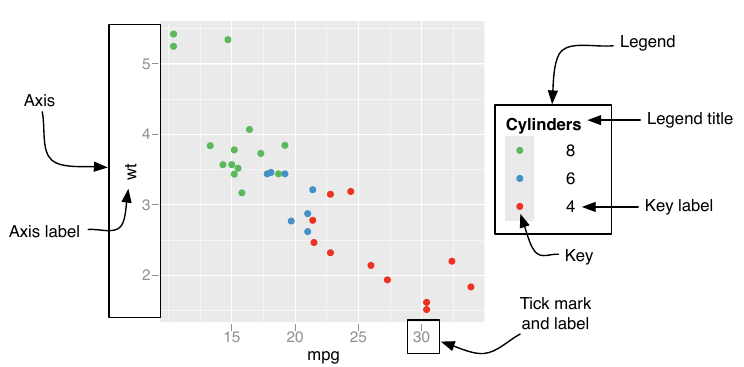
\includegraphics[width=\linewidth]{diagrams/scale-guides}
  \caption{The components of the axes and legend.}
  \label{fig:labelled-guides}
\end{figure}

In ggplot, legends and axes are produced automatically based on the
scales and geoms that you used in the plot. This is different than how
legends work in most other plotting systems, where you are responsible
for adding them. In ggplot, there is little you can do to directly
control the legend. \index{Legend} This seems like a big restriction at
first, but as you get more comfortable with this approach, you will
discover that it saves you a lot of time, and there is little you cannot
do with it.

To draw the legend, the plot must collect information about how each
aesthetic is used: for what data and what geoms. The scale breaks are
used to determine the values of the legend keys and a list of the geoms
that use the aesthetic is used to determine how to draw the keys. For
example, if you use the point geom, then you will get points in the
legend; if you use the lines geom, you will get lines. If both point and
line geoms are used, then both points and lines will be drawn in the
legend. This is illustrated in Figure \ref{fig:legend-geom}.

\begin{figure}

{\centering \includegraphics[width=3.5in]{figures/scaleslegend-geom-1} 

}

\caption{Legends produced by geom: point, line, point and line, and bar.\label{fig:legend-geom}}
\end{figure}

\texttt{ggplot} tries to use the smallest possible number of legends
that accurately conveys the aesthetics used in the plot. It does this by
combining legends if a variable is used with more than one aesthetic.
Figure \ref{fig:legend-merge} shows an example of this for the points
geom: if both colour and shape are mapped to the same variable, then
only a single legend is necessary. In order for legends to be merged,
they must have the same name (the same legend title). For this reason,
if you change the name of one of the merged legends, you'll need to
change it for all of them.

\begin{figure}

{\centering \includegraphics[width=3in]{figures/scaleslegend-merge-1} 

}

\caption{Colour legend, shape legend, colour + shape legend.\label{fig:legend-merge}}
\end{figure}

The contents of the legend and axes are controlled by the scale, and the
details of the rendering are controlled by the theming system. The
following list includes the most commonly tweaked settings.

\begin{itemize}
\itemsep1pt\parskip0pt\parsep0pt
\item
  The scale \texttt{name} controls the axis label and the legend title.
  This can be a string, or a mathematical expression, as described in
  \texttt{?plotmath}.
\item
  The \texttt{breaks} and \texttt{labels} arguments to the scale
  function, introduced earlier in this chapter, are particularly
  important because they control what tick marks appear on the axis and
  what keys appear on the legend. If the breaks chosen by default are
  not appropriate (or you want to use more informative labels), setting
  these arguments will adjust the appearance of the legend keys and axis
  ticks. \index{Legend!keys}
\item
  The theme settings \texttt{axis.*} and \texttt{legend.*} control the
  visual appearance of axes and legends. To learn how to manipulate
  these settings, see \hyperref[sec:themes]{themes}.
\item
  The internal grid lines are controlled by the breaks and minor breaks
  arguments. By default minor grid lines are spaced evenly in the
  original data space: this gives the common behaviour of log-log plots
  where major grid lines are multiplicative and minor grid lines are
  additive. You can override the minor grid lines with the
  \texttt{minor\_breaks} argument. Grid line appearance is controlled by
  the \texttt{panel.grid.major} and \texttt{panel.grid.minor} theme
  settings. \index{Grid}
\item
  The position and justification of legends are controlled by the theme
  setting \texttt{legend.position}, and the value can be right, left,
  top, bottom, none (no legend), or a numeric position. The numeric
  position gives (in values between 0 and 1) the position of the corner
  given by \texttt{legend.justification}, a numeric vector of length
  two. Top right = \texttt{c(1, 1)}, bottom left = \texttt{c(0, 0)}.
  \index{Legend!position}
\end{itemize}

\hyperdef{}{sec:scale-resources}{\section{More
resources}\label{sec:scale-resources}}

As you experiment with different aesthetic choices and new scales, it's
important to keep in mind how the plot will be perceived. Some
particularly good references to consult are:

\begin{itemize}
\itemsep1pt\parskip0pt\parsep0pt
\item
  (Cleveland 1993; Cleveland and McGill 1987; Cleveland 1985) for
  research on how plots are perceived and the best ways to encode data.
\item
  (Tufte 2006; Tufte 1990; Tufte 1997; Tufte 2001) for how to make
  beautiful, data-rich, graphics.
\item
  (Brewer 1994a; Brewer 1994b) for how to choose colours that work well
  in a wide variety of situations, particularly for area plots.
\item
  (Carr and Sun 1999; Carr 1994; Carr 2002) for the use of colour in
  general.
\end{itemize}

Azzalini, A., and A. W. Bowman. 1990. ``A Look at Some Data on the Old
Faithful Geyser.'' \emph{Applied Statistics} 39: 357--65.

Brewer, Cynthia A. 1994a. ``Color Use Guidelines for Mapping and
Visualization.'' In \emph{Visualization in Modern Cartography}, edited
by A.M. MacEachren and D.R.F. Taylor, 123--47. Elsevier Science.

---------. 1994b. ``Guidelines for Use of the Perceptual Dimensions of
Color for Mapping and Visualization.'' In \emph{Color Hard Copy and
Graphic Arts III, Proceedings of the International Society for Optical
Engineering (SPIE), San Jose}, 2171:54--63.

Carr, Dan. 1994. ``Using Gray in Plots.'' \emph{ASA Statistical
Computing and Graphics Newsletter} 2 (5): 11--14.
\url{http://www.galaxy.gmu.edu/~dcarr/lib/v5n2.pdf}.

---------. 2002. ``Graphical Displays.'' In \emph{Encyclopedia of
Environmetrics}, edited by Abdel H. El-Shaarawi and Walter W. Piegorsch,
2:933--60. John Wiley \& Sons.
\url{http://www.galaxy.gmu.edu/~dcarr/lib/EnvironmentalGraphics.pdf}.

Carr, Dan, and Ru Sun. 1999. ``Using Layering and Perceptual Grouping in
Statistical Graphics.'' \emph{ASA Statistical Computing and Graphics
Newsletter} 10 (1): 25--31.

Cleveland, William. 1985. \emph{The Elements of Graphing Data}. Hobart
Press.

---------. 1993. \emph{Visualizing Data}. Hobart Press.

Cleveland, William S, and Robert McGill. 1987. ``Graphical Perception:
The Visual Decoding of Quantitative Information on Graphical Displays of
Data.'' \emph{Journal of the Royal Statistical Society. Series A
(General)} 150 (3): 192--229.

Lumley, Thomas. 2007. \emph{Dichromat: Color Schemes for Dichromats}.

Tufte, Edward R. 1990. \emph{Envisioning Information}. Graphics Press.

---------. 1997. \emph{Visual Explanations}. Graphics Press.

---------. 2001. \emph{The Visual Display of Quantitative Information}.
second. Graphics Press.

---------. 2006. \emph{Beautiful Evidence}. Graphics Press.

Zeileis, Achim, Kurt Hornik, and Paul Murrell. 2008. ``Escaping RGBland:
Selecting Colors for Statistical Graphics.'' \emph{Computational
Statistics \& Data Analysis}.
\url{http://statmath.wu-wien.ac.at/~zeileis/papers/Zeileis+Hornik+Murrell-2008.pdf}.
